\chapter{Del papel a la computadora: discretización}

\begin{enpocas}
Por qué una computadora no puede aplicar una ecuación ``continua'', qué es el periodo de muestreo,
la diferencia entre discretizar de forma explícita e implícita, y por qué esto es el corazón del
proyecto.
\end{enpocas}

\section{La computadora ve a saltos}

Las ecuaciones del capítulo anterior son \emph{continuas}: dicen qué hacer en cada instante. Una
computadora, en cambio, trabaja a pasos: lee los sensores, calcula y manda la orden a los motores, y
repite cada $T_s$ segundos (el \textbf{periodo de muestreo}; en la simulación, 5~ms por omisión, es
decir 200 veces por segundo). Entre una orden y la siguiente, el motor recibe la misma (eso se llama
\textbf{retenedor de orden cero}).

\begin{figure}[H]
\centering
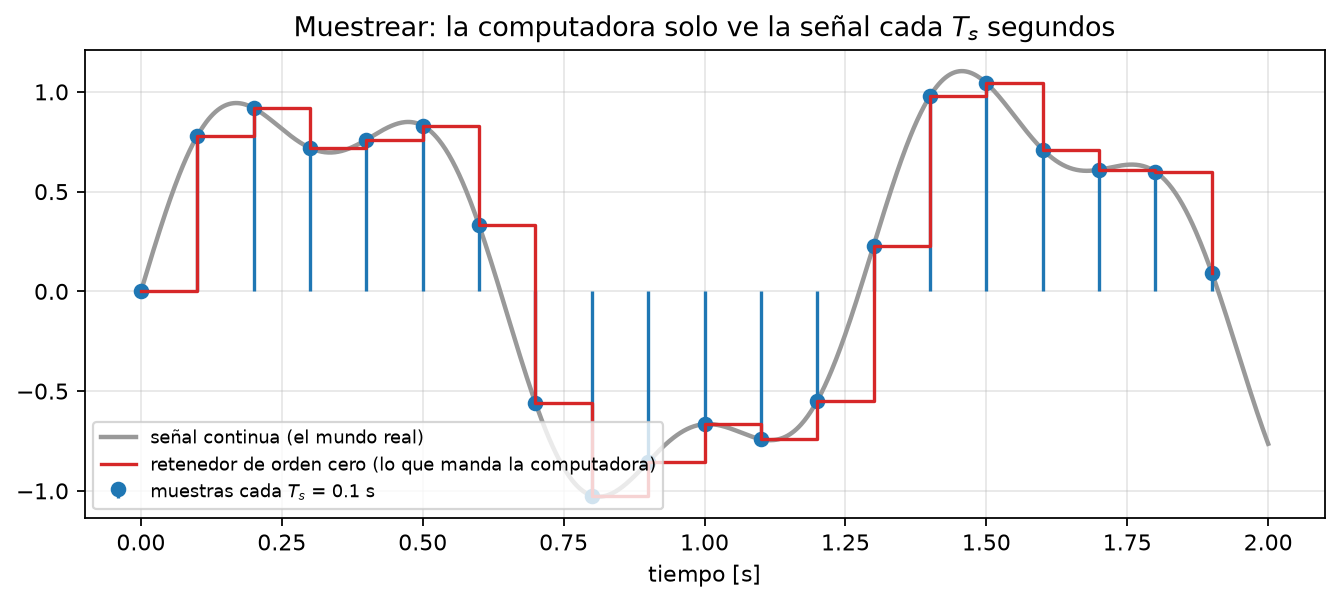
\includegraphics[width=0.9\textwidth]{c_muestreo.png}
\caption{La computadora solo ``ve'' la señal en los instantes de muestreo y mantiene su orden constante
entre ellos.}
\end{figure}

\textbf{Discretizar} es convertir una ley de control continua en una receta de pasos
$k = 0, 1, 2, \dots$ Hay muchas formas de hacerlo y no todas se portan igual.

\section{Un ejemplo para entender: explícito contra implícito}

Tomemos la ecuación más simple que se va a cero: $\dot x = -a x$ (por ejemplo, una taza de café que se
enfría). Con paso $T_s$:

\begin{description}
  \item[Euler explícito] (usar el valor de \emph{ahora}):
        $x_{k+1} = x_k - T_s a\,x_k = (1 - aT_s)\,x_k$.
  \item[Euler implícito] (usar el valor \emph{que va a tener}):
        $x_{k+1} = x_k - T_s a\,x_{k+1} \;\Rightarrow\; x_{k+1} = \dfrac{x_k}{1 + aT_s}$.
\end{description}

Si el paso es pequeño, los dos dan casi lo mismo. Pero si $aT_s > 2$, el explícito multiplica por un
número de valor absoluto mayor que 1 en cada paso: \textbf{explota}, aunque la ecuación original sea
perfectamente estable. El implícito divide siempre por algo mayor que 1: \textbf{nunca explota}.

\begin{figure}[H]
\centering
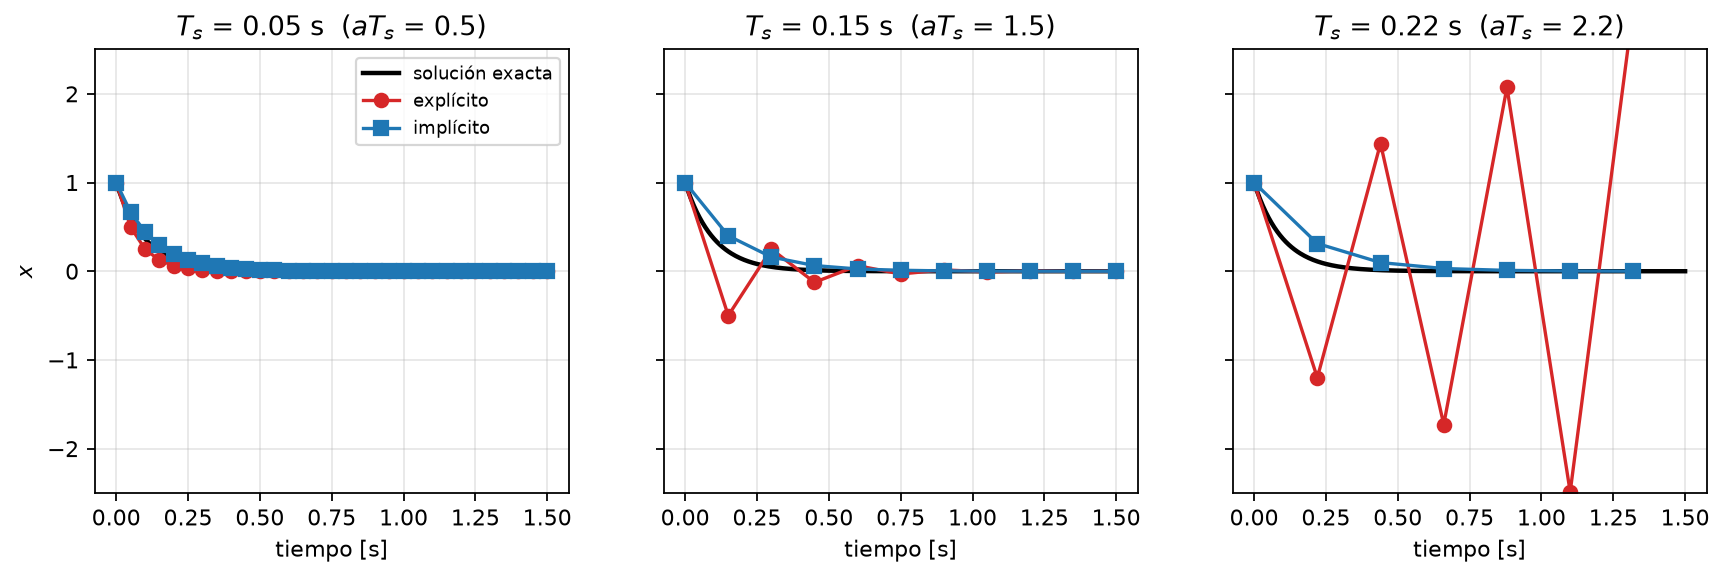
\includegraphics[width=\textwidth]{c_euler.png}
\caption{La misma ecuación $\dot x = -ax$ con $a = 10$, resuelta con pasos cada vez mayores. El
implícito siempre se va a cero; el explícito oscila y, con $aT_s > 2$, diverge.}
\label{fig:euler}
\end{figure}

\begin{recuerda}
\textbf{Explícito}: calculo el siguiente paso con lo que sé ahora; es simple pero puede pasarse.
\textbf{Implícito}: planteo una ecuación con el valor futuro y la resuelvo; cuesta un poco más pero
respeta mejor el comportamiento del sistema continuo.
\end{recuerda}

\section{El problema con los modos deslizantes}

Con la función signo pasa algo parecido, y peor. En la versión explícita del super-twisting:
\begin{equation}
u_k = -k_1|s_k|^{1/2}\sgn(s_k) + \nu_k,\qquad \nu_{k+1} = \nu_k - T_s k_2\sgn(s_k).
\end{equation}
Cerca de $s = 0$, el signo cambia en cada paso y $s$ queda ``rebotando'' alrededor de cero con una
amplitud que crece con la ganancia: es el \textbf{chattering numérico}, producido por la
discretización y no por la física. Y como el STA adaptativo \emph{sube} la ganancia cuando $s$ no está
quieto, el chattering puede alimentar a la adaptación.

\section{La discretización implícita del super-twisting}

La idea (Brogliato, Polyakov y Efimov, 2020) es preguntar: ``¿qué control lleva a $s$ a donde
debería estar en el siguiente paso?'' Se plantea una ecuación con el valor futuro $\tilde s$:
\begin{equation}
\tilde s + T_s k_1|\tilde s|^{1/2}\xi + T_s^2 k_2\,\xi = s_k + T_s\nu_k,\qquad \xi\in\Sgn(\tilde s),
\end{equation}
donde $\Sgn$ es el signo ``como conjunto'': en $\tilde s = 0$ puede valer cualquier número entre $-1$
y $1$. Esa libertad es la clave: si el estado está cerca de la superficie, la ecuación tiene la
solución $\tilde s = 0$ exactamente, con $\xi$ intermedio, en lugar de saltar de $+1$ a $-1$. La
solución se obtiene con una fórmula cerrada (sección~\ref{sec:discretizaciones}).

\begin{figure}[H]
\centering
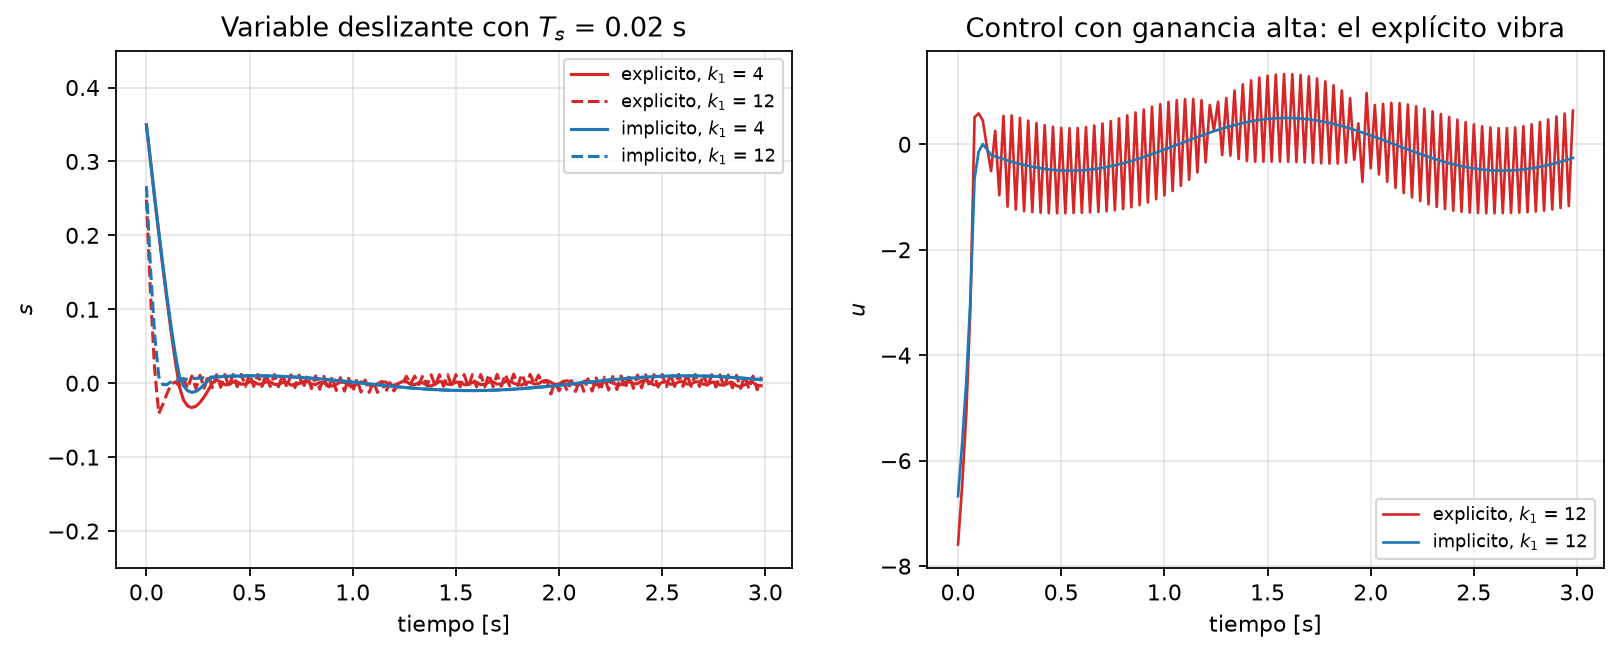
\includegraphics[width=\textwidth]{c_discreto.png}
\caption{Super-twisting con $T_s = 20$~ms y una perturbación senoidal. Con la ganancia alta
($k_1 = 12$), el explícito vibra; el implícito da la misma señal suave que con la ganancia baja.}
\label{fig:discreto}
\end{figure}

\begin{recuerda}
La hipótesis del proyecto: con la discretización implícita, el super-twisting adaptativo conserva su
robustez y elimina el chattering numérico, y deja de ser sensible a que la ganancia sea demasiado
grande. La simulación permite comprobarlo (y ya mostró matices, sección~\ref{sec:observaciones}).
\end{recuerda}

\section{Tres versiones en el código}

\cod{sta.py} implementa las tres, y se elige al lanzar con \cod{esquema:=}:
\begin{description}
  \item[\cod{explicito}] la de arriba;
  \item[\cod{semi_implicito}] el signo se evalúa en el paso siguiente pero la raíz $|s|^{1/2}$ en el
        actual (más fácil de resolver);
  \item[\cod{implicito}] la ecuación completa.
\end{description}

\begin{ejercicio}
Corre la órbita con viento con los tres esquemas y un periodo de muestreo grande, y compara la banda
de $s$ con \cod{metricas.py}:
\begin{lstlisting}[style=bash]
src/cuadrirotor_sim/scripts/corrida.sh ~/corridas/exp.csv 50 esquema=explicito Ts=0.02 k1_0=4.0 adaptativo=false
src/cuadrirotor_sim/scripts/corrida.sh ~/corridas/imp.csv 50 esquema=implicito Ts=0.02 k1_0=4.0 adaptativo=false
src/cuadrirotor_sim/scripts/metricas.py ~/corridas/*.csv
\end{lstlisting}
\end{ejercicio}
